\documentclass[12pt,a4paper]{article}
\usepackage[utf8]{inputenc}
\usepackage[russian]{babel}
\usepackage[OT1]{fontenc}
\usepackage{amsmath}
\usepackage{amsfonts}
\usepackage{amssymb}
\usepackage{graphicx}
\graphicspath{{Images/}}
\usepackage[left=2cm,right=2cm,top=2cm,bottom=2cm]{geometry}
\usepackage{calc}
\usepackage{wrapfig}
\usepackage{setspace}
\usepackage{indentfirst}
\usepackage{subfigure}


\title{
Отчет о выполнении лабораторной работы 1.2.5

Исследование вынужденной регулярной прецессии гироскопа
}

\author{Варламов Антоний, группа Б02-928}

\begin{document}
%Воронцов LaTeX в примерах
\maketitle

\newpage

	\textbf{Цель работы:} исследовать вынужденную прецессию гироскопа; установить зависимость скорости вынужденной прецессии гироскопа от величины момента сил, действующих на ось гироскопа; определить скорость вращения ротора гироскопа и сравнить ее со скоростью, рассчитанной по скорости прецессии.
	
	\textbf{В работе используются:} гироскоп в кардановом подвесе, секундомер, набор грузов, отдельный ротор гироскопа, цилиндр известной массы, крутильный маятник, штангенциркуль, линейка. 


\section{Теоретический материал.}

Основные уравнения движения твердого тела можно записать в виде:

\begin{equation}
	\frac{d\vec{P}}{dt} = \vec{F}
	\label{eq:center_of_mass}
\end{equation}

\begin{equation}
	\frac{d\vec{L}}{dt} = \vec{M}
	\label{eq:moments_equation}
\end{equation}

Формула (\ref{eq:center_of_mass}) выражает закон движения центра масс, а формула (\ref{eq:moments_equation}) -- уравнение моментов, действующих на тело. Двух данных уравнений достаточно для описания состояния твердого тела.

Если сила $\vec{F}$ не зависит от угловой скорости вращения тела, а момент $\vec{M}$ от скорости поступательного движения тела, то уравнения (\ref{eq:center_of_mass}) и (\ref{eq:moments_equation}) можно рассматривать независимо друг от друга. В данной работе рассматривается только задача о вращении твердого тела.

Момент импульса твердого тела можно вычислить, используя формулу:
\begin{equation}
	\vec{L} = \vec{i}I_{x}\omega_{x} + \vec{j}I_{y}\omega_{y} + \vec{k}I_{z}\omega_{z},
\end{equation}
где $ I_{x},I_{y},I_{z} $ -- главные моменты инерции тела, $ \omega_{x}, \omega_{y}, \omega_{z} $ -- компоненты вектора угловой скорости  $\vec{\omega} $.

Быстро вращающееся тело, для которого:

	$$I_{z}\omega_{z} \gg I_{x}\omega_{x}, I_{y}\omega_{y}$$

принято называть \textit{гироскопом}. Гироскоп называется уравновешенным, если его центр масс неподвижен.

В силу (\ref{eq:moments_equation}), приращение момента импулься определяется интегралом:
\begin{equation}
	\Delta\vec{L} =  \int\vec{M}\\,dt
	\label{eq:integral_for_increment}
\end{equation}

Если момент внешних сил действует в течение короткого промежутка времени, из формулы (\ref{eq:integral_for_increment}) следует, что приращение $\vec{L}$ момента импулься значительно меньше самого момента импульса, т.е:

\begin{equation}
	\left| \Delta\vec{L} \right| \ll \left| \vec{L} \right|.
\end{equation}

Благодаря этому, гироскоп приобретает очень большую устойчивость, вызванную его быстрым вращением.

Если гироскоп уравновешен, то суммарный момент сил, действующих на него, равен 0. В таком случае, гироскоп не будет изменять своего положения в пространстве. Если на гироскоп в течение длительного времени будет действовать некоторый момент сил, отличный от нуля, то, согласно (\ref{eq:moments_equation}) гироскоп придет в движение. Мы не будем рассматривать действие моментов сил, которые вызовут ускорение или замедление гироскопа (т.е. моментов сил, которые не изменяют положения оси вращения гироскопа). Рассмотрим действия моментов сил, которые изменяют положение оси вращения гироскопа.

\begin{wrapfigure}[19]{r}{0.4\textwidth}
	\vspace{-2.5ex}
	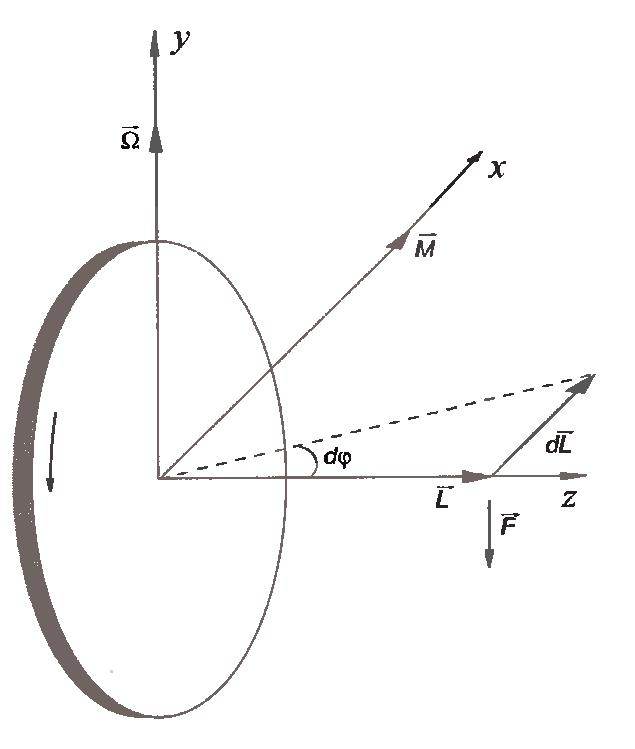
\includegraphics[width = 0.35\textwidth]{flywheel}
	\caption{Маховик.}
	\label{fig:flywheel}
\end{wrapfigure}

Рассмотрим маховик, вращающийся вокруг оси z. (Рис. \ref{fig:flywheel}). Будем считать, что 
$$ \omega_{z} = \omega_{0},\qquad \omega_{x} = \omega_{y} = 0.$$

Пусть ось вращения повернулась в плоскости \textit{zx} по направлению в оси \textit{x} на бесконечно малый угол $d\varphi$. Такой поворот означает добавочное вращение маховика вокруг оси \textit{y}, так что 
$$ d\varphi = \Omega\,dt, $$
где $ \Omega $ -- угловая скорость такого вращения. Будем предполагать, что
\begin{equation}
	L_{\Omega} \ll L_{\omega_{0}}
	\label{eq:condition_for_rotate}
\end{equation}

Это означает, что момент импульса маховика, равный $I_{z}\omega_{0}$ до приложения внешних сил, только повернется в плоскости \textit{zx} по направлению к оси \textit{x} не изменяя своей величины. Таким образом,

\begin{equation}
	\left|d\vec{L}\right| = Ld\varphi = I\Omega\,dt
	\label{eq:increment_moment_of_impulse}
\end{equation}


Записывая выражение (\ref{eq:increment_moment_of_impulse}) в виде векторного произведения, получаем:

\begin{equation}
	\frac{d\vec{L}}{dt} = \vec{\Omega} \times \vec{L}
\end{equation}

Окончательно, используя (\ref{eq:moments_equation}), получаем:

\begin{equation}
	\vec{M} = \vec{\Omega} \times \vec{L}
	\label{eq:rotation_by_moments_of_force}
\end{equation}

Формула (\ref{eq:rotation_by_moments_of_force}) справедлива, если выполнено условие (\ref{eq:condition_for_rotate}).
Данная формула позволяет определить, момент сил $ \vec{M}, $ который нужно приложить к маховику, чтобы вызвать вращение маховика с угловой скоростью $\vec{\Omega}$.

Под действием момента внешних сил $\vec{M}$ ось гироскопа медленно вращается вокруг оси \textit{y} с угловой скоростью $\vec{\Omega}$. Такое движение называют \textit{прецессией гироскопа}.

Для изучения регулярной прецессии уравновешенного гироскопа к его оси подвешивают дополнительные грузы. Это смещает общий центр масс и создает момент сил тяжести, вызывающий прецессию. Скорость прецессии в этом случае может быть найдена по формуле:

\begin{equation}
	\Omega = \frac{mgl}{I_{z}\omega_{0}},
	\label{eq:teor_equation_omega}
\end{equation} 
где m -- масса груза, l -- расстояние от центра карданова подвеса до точки крепления груза на оси гироскопа. (Рис. \ref{fig:facility})

Для выполнения работы используется гироскоп (Рис. \ref{fig:facility}), закрепленный в карданном подвесе (Рис. \ref{fig:Cardan_suspension}).


\begin{figure}[ht!]  
	\vspace{-4ex} 
	\centering 
	\subfigure[]{
		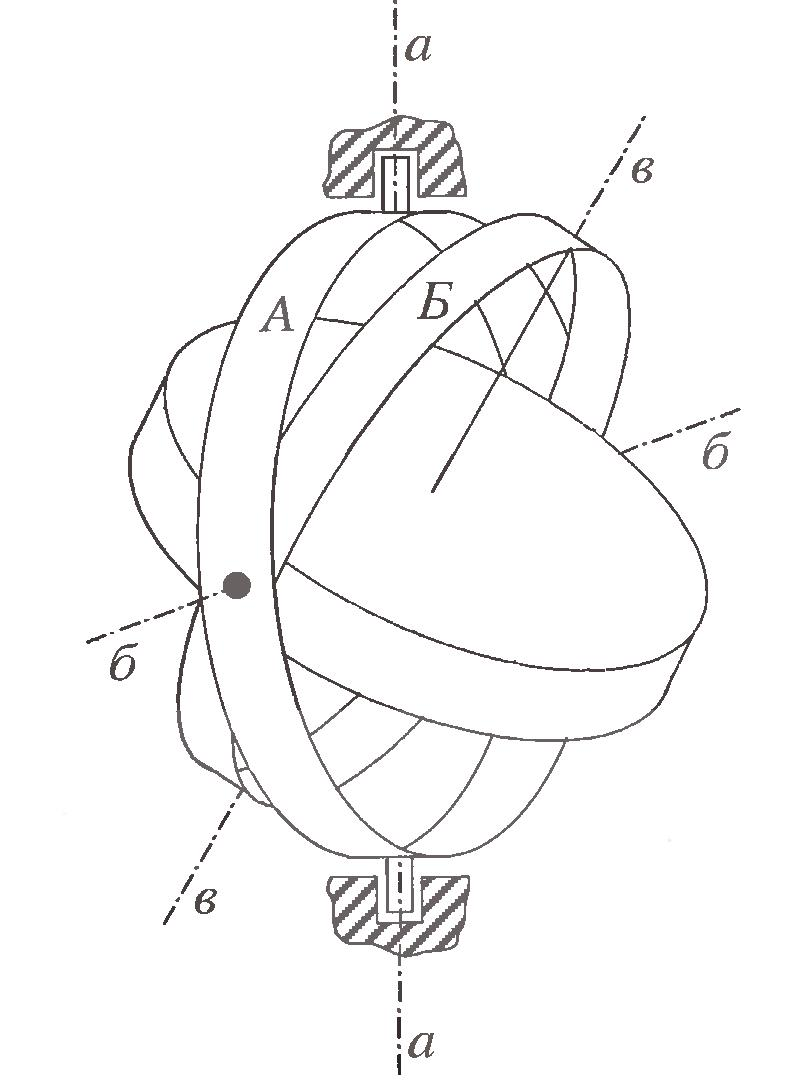
\includegraphics[width=0.29\linewidth]{Cardan_suspension} 	
			\label{fig:Cardan_suspension}}  
	\hspace{4ex}
	\subfigure[]{
		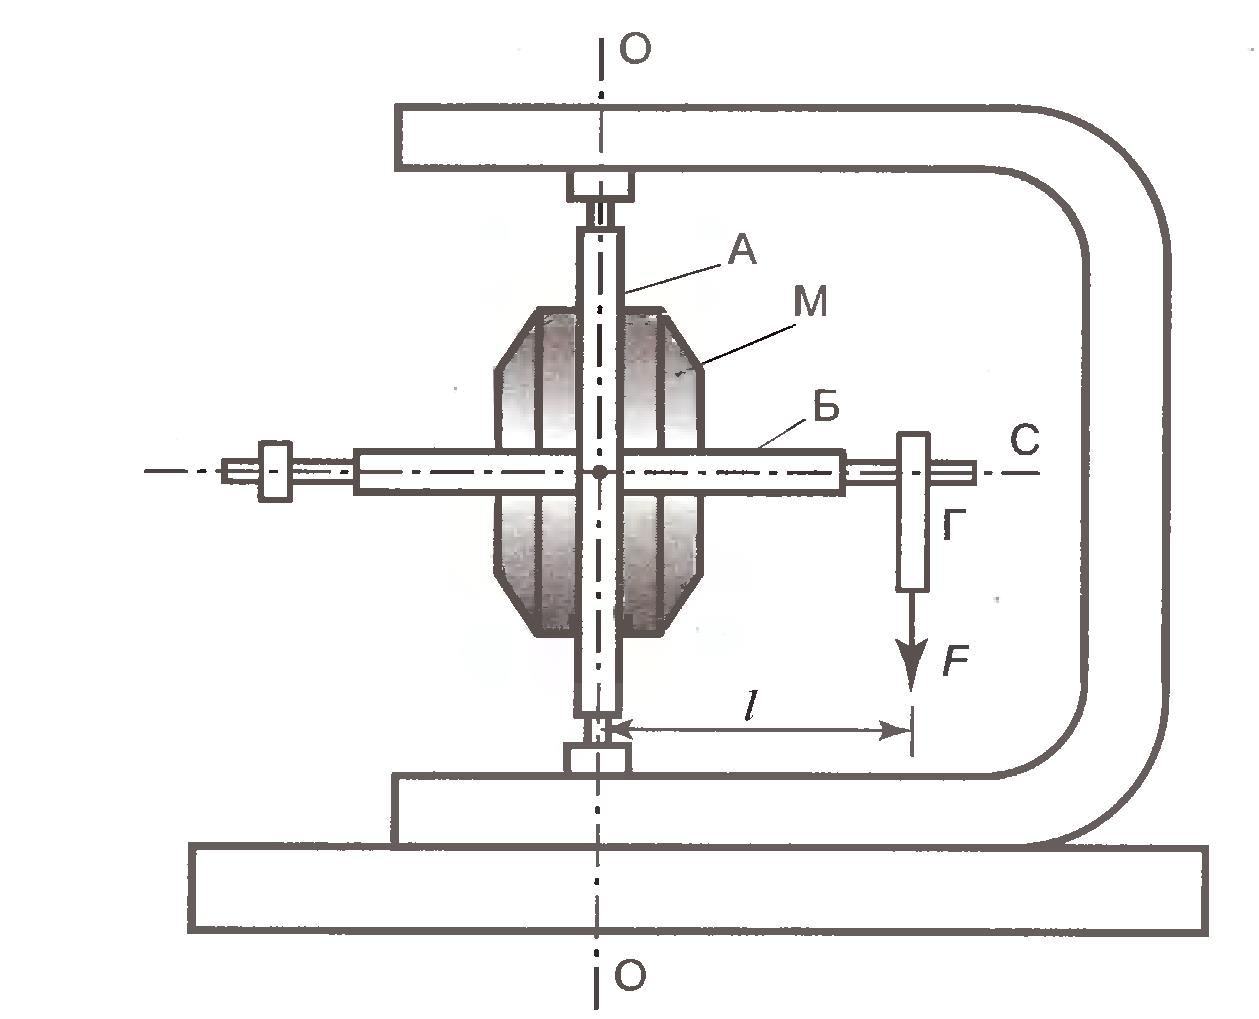
\includegraphics[width=0.45\linewidth]{facility} 
			\label{fig:facility} }  
	\caption{а) Гироскоп, закрепленный в карданном подвесе. б) Схема устройства гироскопа.}
\end{figure}

Ротором гироскопа (Рис. \ref{fig:facility}) является ротор электромотора М. Кожух мотора скреплен с кольцом Б (Рис. \ref{fig:Cardan_suspension}). Мотор с кольцом Б может вращаться в кольце А вокруг горизонтальной оси бб, которое может вращаться относительно оси аа. Рычаг С направлен по оси симметрии ротора. на рычаг подвешивают грузы Г.


\section{Выполнение работы.}
Перед началом работы занесем информацию о грузах, используемых в ходе выполнения работы в Таблицу \ref{tab:load_mass}.

\begin{table}[h!]
	\begin{center}
		\begin{tabular}{|l|l|l|l|l|l|l|l|l|}
			\hline
			№ груза  & 1   & 2   & 3   & 4   & 5   & 6   & 7  & 8  \\ \hline
			Масса, г & 343 & 273 & 220 & 176 & 142 & 116 & 93 & 77 \\ \hline
		\end{tabular}
		\caption{Грузы, используемые в работе.}
		\label{tab:load_mass}
	\end{center}
\end{table}

Перед выполнением работы определим, куда направлен вектор $\vec{\omega}$. Для этого, легким воздействием на рычаг гироскопа вызываем движение его оси. Определяя направление момента прилагаемого усилия, и наблюдая за тем, в каком направлении движется ось, определяем направление момента импульса гироскопа. Так как $\vec{L}\upuparrows \vec{\omega}$, то сразу определяем направление вращения ротора гироскопа. Проведя данный опыт, определяем, что вектор $\vec{\omega}$ направлен в сторону грузов.

\subsection{Измерение периода прецессии оси гироскопа}

	Для измерения периода прецессии оси гироскопа выполним следующие действия. Дав ротору гироскопа раскрутиться, подвешиваем на рычаге, укрепленном на оси гироскопа, груз. Ось гироскопа приходит в движение. Следя за тем, чтобы ось гироскопа опустилась примерно на тот же угол, на который она была отклонена изначально, отмеряем целое или полуцелое число периодов (целое или полуцелое число оборотов оси гироскопа). С помощью секундомера фиксируем время, за которое было совершено это число оборотов. Период прецессии, общее время и число оборотов связанны формулой:
	
	\begin{equation}
		T = \frac{t_{\text{полн}}}{N}
		\label{eq:period_equation}
	\end{equation}
где $t_{\text{полн}}$ -- время, за которое было совершено $N$ оборотов, $N$ -- количество оборотов.

Измерения проведем в виде 5 серий для 8 различных значений внешней силы. (8 различных грузов)

Результаты измерений занесем в таблицу \ref{tab:time_and_count_of_rev}

\begin{table}[h]
	\begin{center}
		\begin{tabular}{|c|c|c|c|c|c|c|c|c|}
			\hline
			\multicolumn{9}{|c|}{I}                                                      \\ \hline
			№ груза & 1      & 2      & 3      & 4      & 5      & 6      & 7      & 8      \\ \hline
			N    & 6      & 5      & 4      & 4      & 4      & 3      & 2      & 2      \\ \hline
			$t_{\text{полное}}$, c    & 212,33 & 222,26 & 220,32 & 274,96 & 344,9  & 314,49 & 261,96 & 318,51 \\ \hline
			T, c & 35,39 & 44,45 & 55,08 & 68,74 & 86,23 & 104,83 & 130,98 & 159,26 \\ \hline
			\multicolumn{9}{|c|}{II}                                                     \\ \hline	
			№ груза & 1      & 2      & 3      & 4      & 5      & 6      & 7      & 8      \\ \hline
			N    & 6      & 5      & 4      & 4      & 4      & 3      & 2      & 2      \\ \hline
			$t_{\text{полное}}$, c     & 212,12 & 222,97 & 220,22 & 275,82 & 344,78 & 314,87 & 262,13 & 318,47 \\ \hline
			T, c & 35,35 & 44,59 & 55,06 & 68,96 & 86,20 & 104,96 & 131,07 & 159,24 \\ \hline
			\multicolumn{9}{|c|}{III}                                                    \\ \hline
			№ груза & 1      & 2      & 3      & 4      & 5      & 6      & 7      & 8      \\ \hline
			N    & 6      & 5      & 4      & 4      & 4      & 3      & 2      & 2      \\ \hline
			$t_{\text{полное}}$, c    & 212,25 & 222,5  & 220,53 & 275,62 & 344,94 & 314,43 & 262,06 & 318,87 \\ \hline
			T, c & 35,38 & 44,50 & 55,13 & 68,91 & 86,24 & 104,81 & 131,03 & 159,44 \\ \hline
			\multicolumn{9}{|c|}{IV}                                                     \\ \hline
			№ груза & 1      & 2      & 3      & 4      & 5      & 6      & 7      & 8      \\ \hline	
			N    & 6      & 5      & 4      & 4      & 4      & 3      & 2      & 2      \\ \hline
			$t_{\text{полное}}$, c    & 212,09 & 222,56 & 220,31 & 274,79 & 345,03 & 314,2  & 262,31 & 318,4  \\ \hline
			T, c & 35,35 & 44,51 & 55,08 & 68,70 & 86,26 & 104,73 & 131,16 & 159,20 \\ \hline
			\multicolumn{9}{|c|}{V}                                                      \\ \hline
			№ груза & 1      & 2      & 3      & 4      & 5      & 6      & 7      & 8      \\ \hline
			N    & 6      & 5      & 4      & 4      & 4      & 3      & 2      & 2      \\ \hline
			$t_{\text{полное}}$, c & 212,44 & 222,16 & 220,42 & 275,02 & 345,1  & 314,67 & 262,12 & 318,32 \\ \hline
			T, c & 35,41 & 44,43 & 55,11 & 68,76 & 86,28 & 104,89 & 131,06 & 159,16 \\ \hline
		\end{tabular}
		\caption{Результаты измерения времени и количества оборотов оси гироскопа при его прецессии. Значение периодов вынужденной прецессии гироскопа}
		\label{tab:time_and_count_of_rev}
	\end{center}
\end{table}



Используя полученные значения периодов прецессии, определим $T, \sigma_{T}, \varepsilon_{T}$, результаты занесем в Таблицу \ref{tab:periods_and_sigma}.

\begin{table}[h]
	\begin{center}
		\begin{tabular}{|c|c|c|c|c|c|}
			\hline
			№ груза & $T$ & $\sigma_{\text{сист}}$ & $\sigma_{\text{случ}}$ & $\sigma_{T}$ & $\varepsilon_{T}$ \\ \hline
			1       & 35,37  & 0,01       & 0,02       & 0,03  & 0,0007  \\ \hline
			2       & 44,50  & 0,01       & 0,06       & 0,06  & 0,0014  \\ \hline
			3       & 55,09  & 0,01       & 0,03       & 0,03  & 0,0006  \\ \hline
			4       & 68,81  & 0,01       & 0,11       & 0,11  & 0,0016  \\ \hline
			5       & 86,24  & 0,01       & 0,03       & 0,03  & 0,0004  \\ \hline
			6       & 104,84 & 0,01       & 0,08       & 0,08  & 0,0008  \\ \hline
			7       & 131,06 & 0,01       & 0,06       & 0,06  & 0,0005  \\ \hline
			8       & 159,26 & 0,01       & 0,11       & 0,11  & 0,0007  \\ \hline
		\end{tabular}
		\caption{Период прецессии для различных грузов.}
		\label{tab:periods_and_sigma}
	\end{center}
\end{table}

Как можно заметить из таблицы \ref{tab:periods_and_sigma}, величина относительной погрешности измерения периода прецессии достаточно мала. определим по полученным данным величину $\Omega$. Для этого воспользуемся формулой:

\begin{equation}
	\Omega = \frac{2\pi n \pm \Delta\varphi}{t_{\text{полн}}}
	\label{eq:definition_Omega}
\end{equation} 
	
	Применив формулу \ref{eq:definition_Omega} к данным таблицы \ref{tab:periods_and_sigma} и занесем результат в Таблицу \ref{tab:first_experimental_Omega}.На основе данных таблицы построим график, изображенный на рисунке \ref{fig:graphic_Omega_moment}.
	
\begin{table}[h!]
	\centering
	\begin{tabular}{|c|c|c|c|c|c|c|c|c|}
		\hline
		№ груза & 1      & 2      & 3      & 4      & 5      & 6      & 7      & 8      \\ \hline
		$\Omega$,рад/c   & 0,1776 & 0,1412 & 0,1141 & 0,0913 & 0,0729 & 0,0599 & 0,0479 & 0,0395 \\ \hline
	\end{tabular}
	\caption{Значения угловой скорости для различных грузов.}
	\label{tab:first_experimental_Omega}
\end{table}

\begin{figure}[h!]
	\begin{center}
		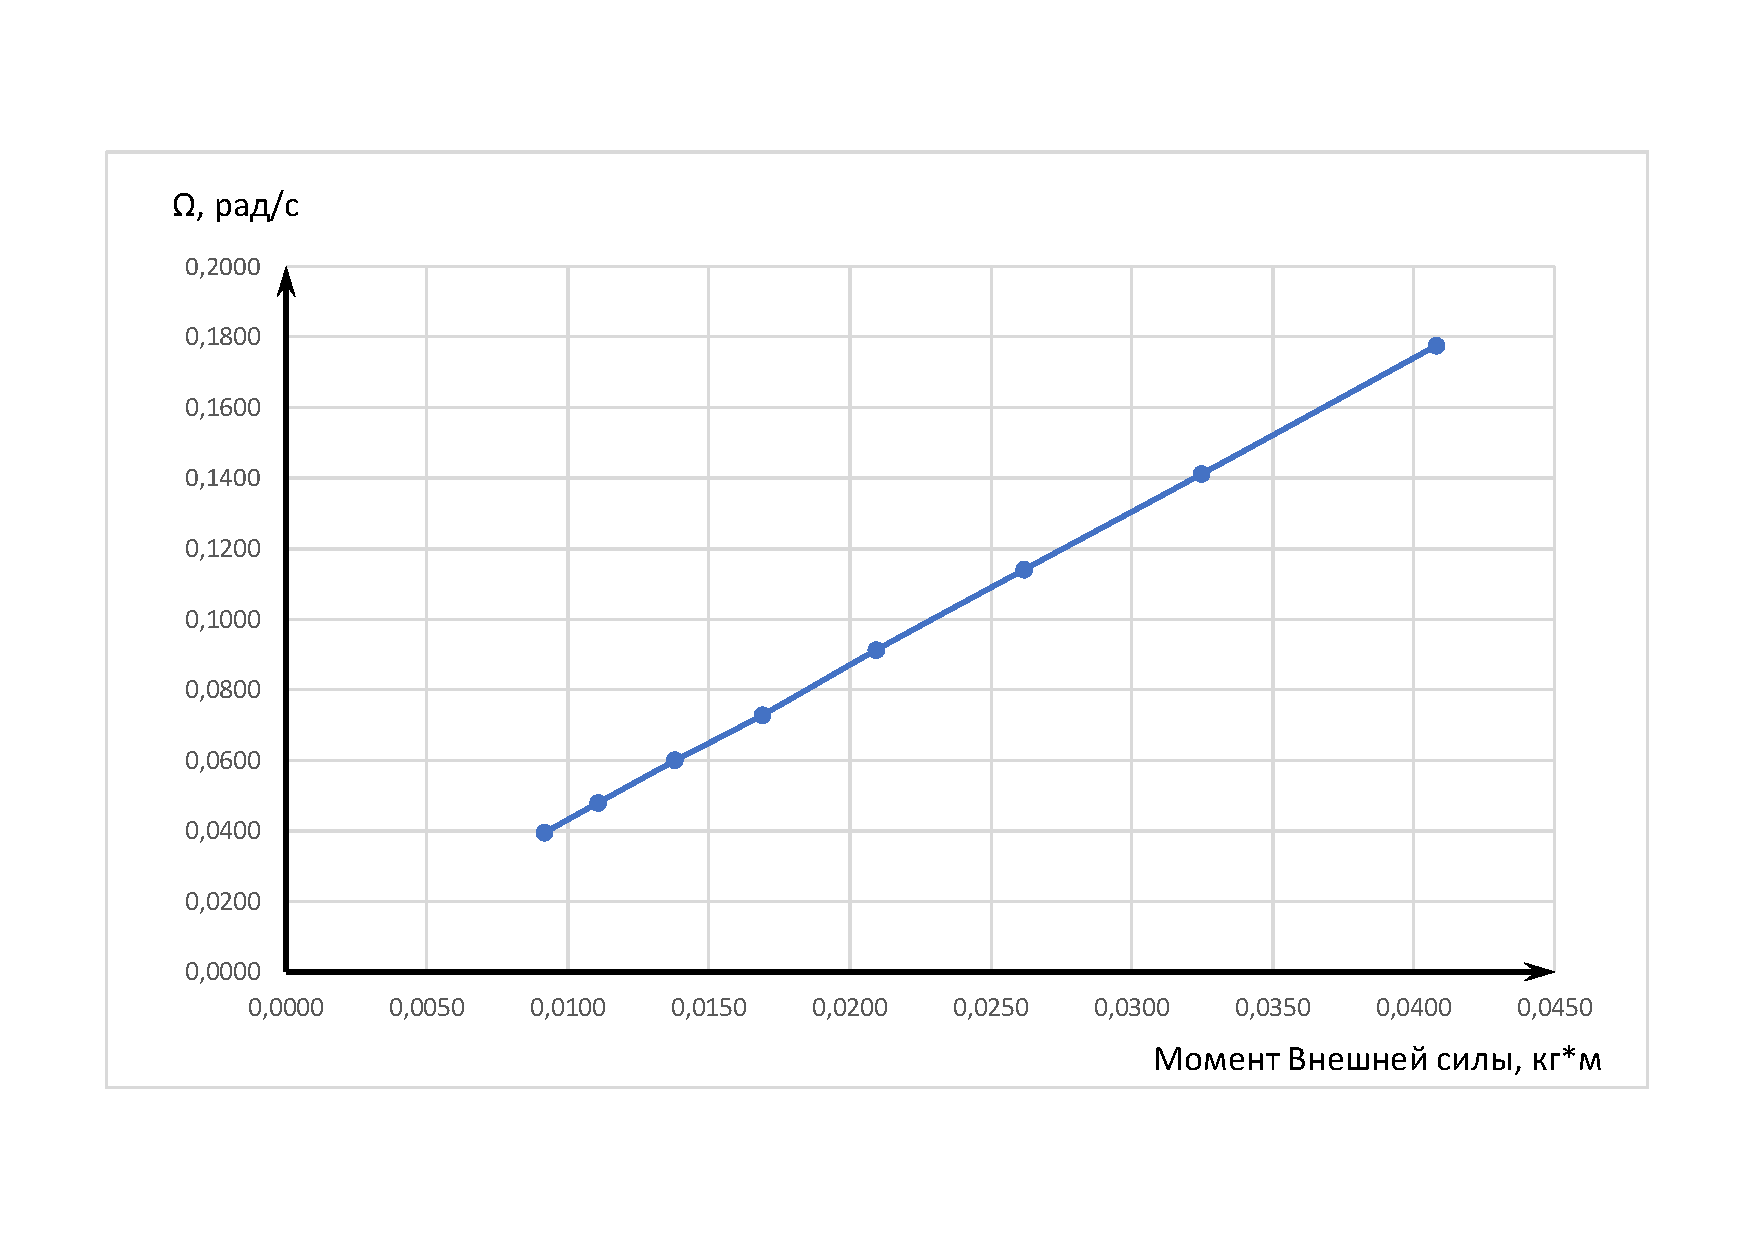
\includegraphics[width = 0.95\textwidth]{Omega_moments_graphic}
		\caption{График зависимости $\Omega(M)$}
		\label{fig:graphic_Omega_moment}
	\end{center}
\end{figure}

\newpage

\subsection{Измерение момента инерции ротора гироскопа}

Следующим этапом выполнения работы будет определение момента инерции ротора гироскопа. Для этого мы используем метод крутильных колебаний. Для определения момента инерции ротора гироскопа используем формулу:

\begin{equation}
	I_{\text{ротора}}= I_{\text{ц}}\frac{T_{\text{ротора}}^2}{T_{\text{ц}}^2},
	\label{eq:moment_measuring_equation}
\end{equation}
где $I_{\text{ц}}$ -- момент инерции цилиндра, $T_{\text{ротора}}$ -- период крутильных колебаний ротора гироскопа, $T_{\text{ц}}$ -- период крутильных колебаний цилиндра.

Произведем измерение данных величин.
Измерения периодов колебаний будем проводить, отсчитывая 30 полных колебаний. Полученные результаты занесем в таблицу \ref{tab:results_of_measuring}

\begin{table}[h!]
	\centering
		\begin{tabular}{|l|l|l|}
			\hline
			Величина 			 & значение & $\sigma$    \\ \hline
			$30T_{0}$, c  			 & 96,88    & 0,1         \\ \hline
			$30T_{\text{ц}}$, c  			 & 122,51   & 0,1         \\ \hline
			$M_{\text{ц}}$, г    & 1617,8   & 0,1         \\ \hline
			$R_{\text{ц}}$, мм   & 39       & 0,25        \\ \hline
		\end{tabular}
		\caption{Результаты измерения}
		\label{tab:results_of_measuring}
\end{table}

Используя формулу \ref{eq:moment_measuring_equation} и данные таблицы \ref{tab:results_of_measuring} получим итоговые значения, занесенные в таблицу \ref{tab:results_of_measuring_moment}.

Величины $\varepsilon_{T}, \varepsilon_{I_{\text{ц}}}, \varepsilon_{I_{0}}$ рассчитываются по следующим формулам:

\begin{equation}
	\varepsilon_{T} = \frac{\sigma_{T}}{T}
\end{equation}	

\begin{equation}
	\varepsilon_{I_{\text{ц}}} = \left(\frac{\sigma_{M}}{M}\right) + 2\left(\frac{\sigma_{R}}{R}\right)
\end{equation}	

\begin{equation}
	\varepsilon_{I_{0}} = \varepsilon_{I_{\text{ц}}} + \varepsilon_{T_{0}} + \varepsilon_{T_{\text{ц}}}
\end{equation}

\begin{table}[h!]
	\centering
	\begin{tabular}{|c|c|c|c|}
		\hline
		 Величина     & Значение    & $\sigma$   & $\varepsilon$  \\ \hline
		$T_{0}, c$   & 3,23    & 0,003   & 0,001    \\ \hline
		$T_{\text{ц}}, c$  & 4,08    & 0,003   & 0,001    \\ \hline
		$I_{\text{ц}}, \text{кг}\cdot \text{м}^{2}, \cdot 10^{-4}$  & 12,3 & 0,2 & 0,013 \\ \hline
		$I_{\text{0}}, \text{кг}\cdot \text{м}^{2}, \cdot 10^{-4}$ & 7,7 & 0,1 & 0,017 \\ \hline
	\end{tabular}
	\caption{Результаты измерений момента инерции ротора гироскопа}
	\label{tab:results_of_measuring_moment}
\end{table}

В итоге, полученное значение момента инерции ротора цилиндра:

\begin{equation}
	I_{0} = \left( 7,7 \pm 0,1 \right) \cdot 10^{-4}\quad \text{Кг} \cdot \text{м}^{2}
	\label{eq:moment_of_inertion_result}
\end{equation} 

Используя величину \ref{eq:moment_of_inertion_result} и формулу \ref{eq:teor_equation_omega} определим величины угловой скорости для каждого из грузов. Значения занесем в таблицу \ref{tab:teor_result_Omega_for_diffrent_frequency}.

\begin{table}[h!]
	\centering
		\begin{tabular}{|c|c|c|c|c|c|c|c|c|}
			\hline
			\multicolumn{9}{|c|}{$\nu=460$ Гц}                                                   \\ \hline
			груз         & 1      & 2      & 3      & 4      & 5      & 6      & 7      & 8      \\ \hline
			$\Omega$, рад/с & 0,1800 & 0,1433 & 0,1154 & 0,0924 & 0,0745 & 0,0609 & 0,0488 & 0,0404 \\ \hline
			\multicolumn{9}{|c|}{$\nu=490$ Гц}                                                   \\ \hline
			груз         & 1      & 2      & 3      & 4      & 5      & 6      & 7      & 8      \\ \hline
			$\Omega$, рад/с & 0,1690 & 0,1345 & 0,1084 & 0,0867 & 0,0700 & 0,0572 & 0,0458 & 0,0379 \\ \hline
		\end{tabular}
		\caption{Значение угловых скоростей прецессии оси гироскопа в зависимости от груза для двух полученных 	значений частоты вращения ротора гироскопа}
		\label{tab:teor_result_Omega_for_diffrent_frequency}
\end{table}
 
Значения частот вращения ротора гироскопа будут получены в пункте \ref{subsec:def_of_frequency}.
Кроме того, в пункте \ref{subsec:def_of_frequency} будет определяться, какая из двух полученных частот наиболее близка к реальности. Для этого изобразим графики 3 зависимостей $\Omega(M)$ -- экспериментальной и 2 теоретических: для значений частот 460 и 490 Гц. Полученные зависимости изображены на графике \ref{fig:diffrent_dependence_Omega}.

\begin{figure}[h!]
	\begin{center}
		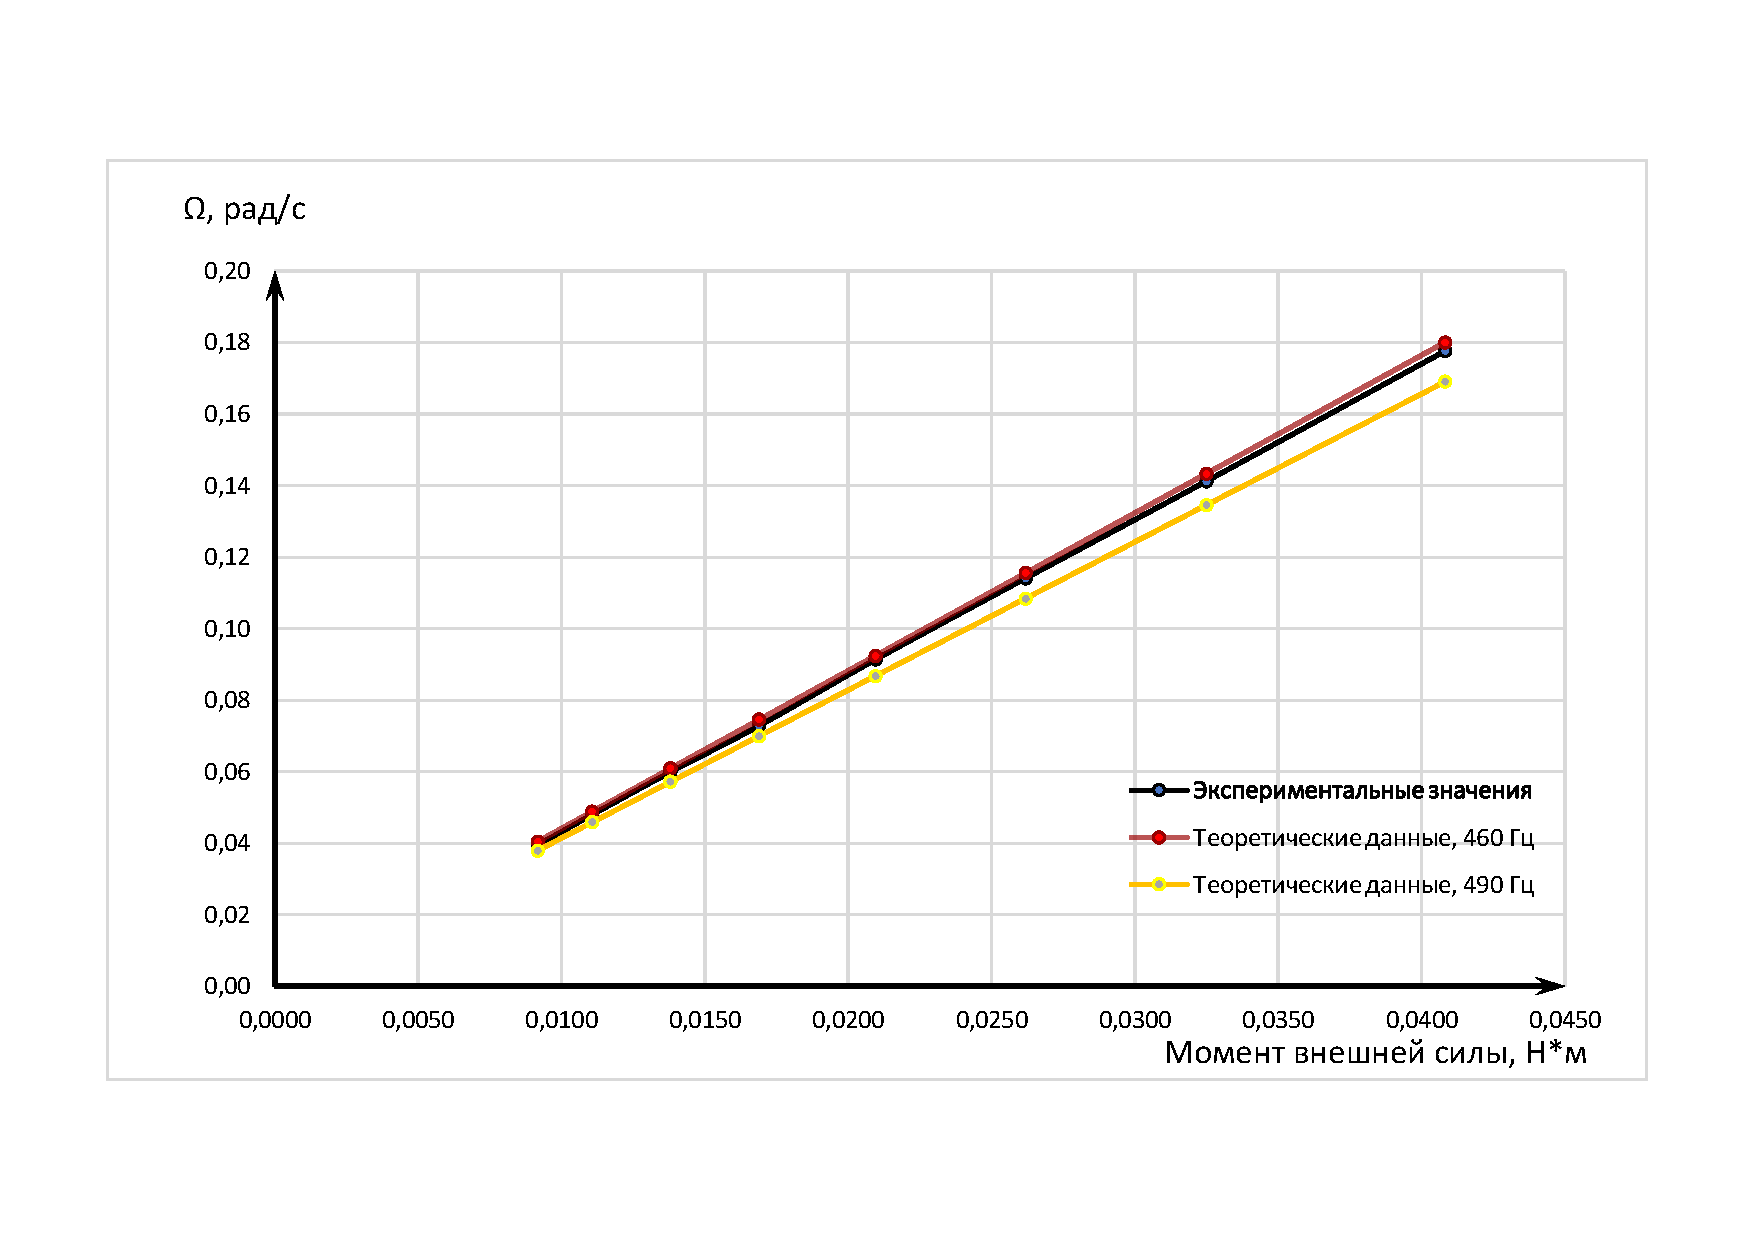
\includegraphics[width = 0.95\textwidth]{Diffrent_Omega(M)_dependence_graphic_color}
		\caption{Графики зависимости $\Omega(M) для разлличных данных$}
		\label{fig:diffrent_dependence_Omega}
	\end{center}
\end{figure}

\subsection{Измерение момента сил трения в оси карданного подвеса}
В данном пункте определим момент сил трения, возникающих в осях карданного подвеса, в котором закреплен гироскоп.
Для этого определим скорость прецессии оси гироскопа в вертикальной плоскости. 

Для определения скорости прецессии используем формулу:
\begin{equation}
	\Omega_{\text{верт}} = 2\alpha/t_{all},
	\label{eq:Omega_vertical}
\end{equation}
где $t_{all}$ -- время, за которое произошло опускание, $\alpha$ -- начальный угол, на который отклонена ос гироскопа от горизонтальной плоскости.

В качестве времени возьмем среднее значении времен, используемых для определения периодов регулярной прецессии
Кроме того, определим значения угла $\alpha$, на который изначально отклонялась ось гироскопа при своем вращении.

Значение времени: $t = 254 $с;

Величину момента сил трения можно определить по следующей формуле:

\begin{equation}
	M_{F_{\text{трения}}} = 2\pi\Omega I_{0}\omega_{z}
\end{equation}

Используя формулу $\ref{eq:Omega_vertical}$, получаем:

\begin{equation}
	M_{F_{\text{трения}}} = \frac{4\pi I_{0}\omega_{z}\arctan\left(\frac{\Delta h}{l}\right)}{t_{\text{полн}}}
	\label{eq:moment_of_force_sopr}
\end{equation}

Используя формулу \ref{eq:moment_of_force_sopr} и полученные ранее значения входящих в нее величин, можем оценить величину момента сил трения, возникающих в оси карданного подвеса:

\begin{equation}
	M_{F_{\text{трения}}} = 2,2 \cdot 10^{-4} \quad\text{Н}\cdot\text{м}
\end{equation}

Определим погрешность полученного результата. 

\begin{equation}
	\sigma_{M} = \sqrt{\varepsilon_{\alpha}^{2} + \varepsilon_{I_{0}}^{2} + \varepsilon_{\omega_{z}}^{2} + \varepsilon_{t_{\text{полн}}}^{2}}
\end{equation}

\begin{equation}
	\sigma_{\alpha} = \frac{\partial \alpha}{\partial \frac{\Delta h}{l}} = \frac{\sigma_{\frac{\Delta h}{l}}}{1 + \frac{\Delta h}{l}}
\end{equation}

В итоге:

\begin{equation}
	M = (2,2 \pm 0,3)\cdot 10^{-4}\quad \text{Н}\cdot\text{м}
\end{equation}

\subsection{Определение частоты вращения ротора гироскопа с помощью фигур Лиссажу} \label{subsec:def_of_frequency}

Для определения частоты вращения ротора гироскопа воспользуемся электронным осциллографом с генератором. На один вход генератора подается сигнал с генератора, а к другому подключен ротор гироскоп. Выключая режим развертки на осциллографе и настраивая частоту выходного сигнала генератора добиваемся картины невырожденного эллипса на экране осциллографа. Если на экране получен эллипс, то частота входного сигнала, идущего от генератора, равна частоте вращения ротора генератора. Проводя данные действия в 2 случаях (со включенным и с выключенным гироскопом соответственно), были получены два значения частоты: 490 Гц и 460 Гц соответственно. Необходимо определить, какая из двух данных частот наиболее близка к реальной частоте вращения ротора гироскопа. Для этого обратимся к графику \ref{fig:diffrent_dependence_Omega}. На приведенном графике видно, что прямая, наилучшим образом приближающая экспериментальные данные, полученные ранее, это прямая, которая соответствует значению частоты вращения ротора равной 460 Гц. В итоге, можно сказать, что наиболее точное значение частоты вращения ротора гироскопа можно получить при проведении измерения сразу после выключения гироскопа от сети. Для подтверждения данного факта, сравним отклонения для двух зависимостей. Полученные результаты занесем в Таблицу \ref{tab:deflection}.



\begin{table}[h!]
\centering
\resizebox{\textwidth}{!}{%
\begin{tabular}{|c|c|c|c|c|}
\hline
\begin{tabular}[c]{@{}c@{}}Значения $\Omega$\\  для экспериментальных \\ данных\end{tabular} & \begin{tabular}[c]{@{}c@{}}Значения $\Omega$\\  для частоты вращения\\ ротора, равной 460  Гц, рад/с\end{tabular} & \begin{tabular}[c]{@{}c@{}}Значения\\ для частоты вращения\\ ротора, равной 490  Гц, рад/с\end{tabular} & $\delta_{\Omega_{\text{экс}} - \Omega_{\text{теор; 460 Гц}}}$ & $\delta_{\Omega_{\text{экс}} - \Omega_{\text{теор; 490 Гц}}}$ \\ \hline
0,1776                                                                           & 0,1801                                                                                          & 0,1690                                                                                         & 0,002 & 0,009 \\ \hline
0,1412                                                                           & 0,1433                                                                                          & 0,1345                                                                                         & 0,002 & 0,007 \\ \hline
0,1141                                                                           & 0,1155                                                                                          & 0,1084                                                                                         & 0,001 & 0,006 \\ \hline
0,0913                                                                           & 0,0924                                                                                          & 0,0867                                                                                         & 0,001 & 0,005 \\ \hline
0,0729                                                                           & 0,0745                                                                                          & 0,0700                                                                                         & 0,002 & 0,003 \\ \hline
0,0599                                                                           & 0,0609                                                                                          & 0,0572                                                                                         & 0,001 & 0,003 \\ \hline
0,0479                                                                           & 0,0488                                                                                          & 0,0458                                                                                         & 0,001 & 0,002 \\ \hline
0,0395                                                                           & 0,0404                                                                                          & 0,0379                                                                                         & 0,001 & 0,002 \\ \hline
\end{tabular}%
}
\caption{Значения для различных теоретических данных и их отклонения от экспериментальных значений.}
\label{tab:deflection}
\end{table}

Как видно из Таблицы \ref{tab:deflection}, теоретическая зависимость при значении частоты вращения ротора 460 Гц описывает экспериментальные данные лучше, чем теоретическая зависимость при значении частоты 490 Гц.

Подтвердим полученный результат, оценив частоту вращения ротора гироскопа с помощью теоретических формул. Результаты занесем в Таблицу \ref{tab:mnk_for_omega}.

\begin{table}[h]
\centering
\begin{tabular}{|c|c|c|c|c|c|c|c|c|}
\hline
№ груза & 1        & 2       & 3        & 4        & 5        & 6        & 7        & 8        \\ \hline
$\omega$, рад/с   & 469 & 469 & 468 & 468 & 473 & 470 & 471 & 474 \\ \hline
\end{tabular}
\caption{Значения угловой скорости вращения ротора, определенные по теоретической формуле.}
\label{tab:mnk_for_omega}
\end{table}

Определив $\sigma_{\omega}$ с помощью МНК, получаем:

\begin{equation}
	\sigma_{\omega} = 4 \text{рад/с}
\end{equation}

Итоговое значение частоты вращения ротора гироскопа:

\begin{equation}
	\omega_{z} = 471 \pm 4 \text{рад/с}
\end{equation}

\subsection{Сравнение полученных результатов}

В итоге, в ходе выполнения работы были получены следующие результаты:

Значения $\Omega$ представлены в таблице \ref{tab:final_table};

\begin{table}[h!]
\centering
\begin{tabular}{|c|c|}
\hline
$\Omega_{\text{теоретическая}}$, рад/с & $\Omega_{\text{экспериментальная}}$, рад/с \\ \hline
0,1801              & 0,1776                  \\ \hline
0,1433              & 0,1412                  \\ \hline
0,1155              & 0,1141                  \\ \hline
0,0924              & 0,0913                  \\ \hline
0,0745              & 0,0729                  \\ \hline
0,0609              & 0,0599                  \\ \hline
0,0488              & 0,0479                  \\ \hline
0,0404              & 0,0395                  \\ \hline
\end{tabular}
\caption{Значения угловой скорости оси маятника во время прецессии определенные теоретически и экспериментально}
\label{tab:final_table}
\end{table}
 
Значение момента инерции ротора гироскопа: $I_{0} = \left( 7,7 \pm 0,1 \right) \cdot 10^{-4}\quad \text{Кг} \cdot \text{м}^{2}$;

Значение момента сил трения в оси карданного подвеса : $M = (2,2 \pm 0,5)\cdot 10^{-4}\quad \text{Н}\cdot\text{м}$
\newpage
\section{Результаты}
\begin{enumerate}
	\item В ходе выполнения работы были определены физические величины, описывающие регулярную прецессию гироскопа, закрепленного в карданном подвесе, а именно:
		\begin{itemize}
			\item Была определена теоретически и экспериментально угловая скорость регулярной прецессии гироскопа: Таблица \ref{tab:final_table}. Полученная точность теоретически определенной величины совпадает с точностью, с которой можно определить момент инерции ротора гироскопа, так как эта величина вносит наибольший вклад в погрешность. Достигнутая точность: $\varepsilon_{\Omega_{\text{теоретическая}}} = 0,013$. Оценить точность измерения экспериментального значения $\varepsilon_{\Omega_{\text{экспериментальная}}}$ можно только достаточно грубо, с учетом величины $\delta \varphi$?, используемой в качестве погрешности определения числа оборотов оси гироскопа. С учетом этого величина $\varepsilon_{\Omega_{\text{экспериментальная}}} \approx 0,028$.
			\item Был определен момент инерции ротора гироскопа: $I_{0} = \left( 7,7 \pm 0,1 \right) \cdot 10^{-4}\quad \text{Кг} \cdot \text{м}^{2}$; Точность определения: $\varepsilon_{I_{0}} = 0,013$; Основной вклад -- погрешность измерения радиуса цилиндра, с помощью которого определялась данная величина.
			\item Был определен момент сил трения, возникающих в оси карданного подвеса: $M = (2,2 \pm 0,3)\cdot 10^{-4}\quad \text{Н}\cdot\text{м}$; Достигнута точность:  $\varepsilon_{M} = 0,14$; Основной вклад: погрешность измерения угла отклонения оси от горизонтальной плоскости, погрешность фиксирования прохождения оси через начальную точку.
		\end{itemize}
	\item На практике были подтверждены все теоретические зависимости, используемые в данной работе.
	\item Показано соответствие различных методов определения физических величин : угловая скорость, частота.
	\item Достигнута приемлемая точность. (Максимальное значение относительной погрешности среди всех измерений - $\varepsilon_{M_{F_{\text{трения}}}} = 0,14$)
\end{enumerate}

\end{document}
